\begin{figure}[b!]
\centering
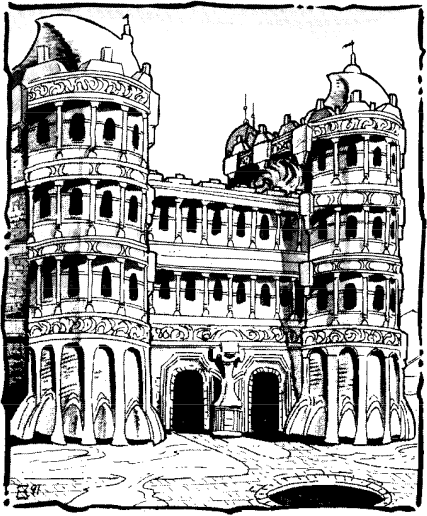
\includegraphics[width=\columnwidth]{images/urik-1.png}
\par\textit{\small\textcopyright Wizards of the Coast, 2020.}
\end{figure}

\City{Urik}
{30,000 (75\% humans, 10\% half-giants, 5\% dwarves, 3\% muls, 3\% thri-kreen, 2\% elves, 1\% halfling, 1\% other).}
{Obsidian, silk, pottery.}
{Common, Dwarven, Urikite.}
{
	Located northeast of Tyr, between the Dragon's Bowl and the Smoking Crown Mountains, the square, clean lines of the city-state of Urik can be found. The city-state has remained virtually the same as it was before the Great Earthquake and the demise of the Dragon. Hamanu, the King of the World and the Lion of Urik, was away from his city when the tremor struck.

	Although minor damage and only a few deaths resulted from the quake, the citizens trembled. When Hamanu returned, he promised his citizens that they would have nothing else to fear from Athas and its cruel temperament. The sorcerer-king's word (and his magic) was as strong as precious steel, for neither the aftershocks nor the Tyr-storm that arrived two months later could breach the towering yellow walls of Urik.

	Hamanu's promise wasn't unconditional. Though the Urikites don't have to fear change, they do have to fear their king. To disobey Hamanu is to risk punishment and even death, while to obey him is to live without fear. That's how it's always been in eternal Urik, and that's how it always will be.

	Urikites wear their hair in square cuts with elaborate ringlets. Some men wear square-cut curled beards. White linen shirts with short, tight sleeves are the fashion of Urik. Individuals of the lower classes wear plain, unadorned shirts that fall to their knees. Individuals of the upper classes increase the length to their ankles and add a striped or diamond pattern as well as a tassel-trimmed girdle. Elaborate scarves, worn only at night, indicate a citizen's station. The longer and richer the scarf, the higher the wearer's social status. By law and tradition, only templars may wear cloaks, and these are always bleached pure white for the low to mid levels and tinged yellow for the higher ranks.
}
{
	Except for the new restrictions regarding trade and travel, things in Urik are the same as they ever were. The city remains a warrior culture, ruled by a warrior king and geared toward fighting and winning wars. The current enemies aren't the other city-states, however. Rather, the refugees seeking shelter from the constant tremors and the monsters fleeing from the violent storms near the Silt Sea have become Urik's foes. When either approaches Urik's high, yellow walls, Hamanu leads his army out of his gigantic palace (called Destiny's Kingdom) and charges into battle. In most cases, the result is slaughter, for terrified invaders can't stand against Hamanu's highly trained and well-equipped legions.

	The few signs that the Great Earthquake touched Urik have been wiped out; buildings have been repaired, streets repaved, the dead buried. Now, Hamanu's magic keeps the aftershocks and the storms from entering the city, and in most respects the citizens have learned to ignore the disasters. As long as the disasters remain outside Urik's walls, the citizens see no reason to worry about them.

	Closing the city off from the rest of the world has made it difficult for certain members of Urik's society. Adventurers and traders, for example, are severely hampered by the well-guarded walls. Elves, never really welcome near Urik's walls, now avoid the city completely. They are treated like invaders, set upon as soon as they're spotted entering Urik's verdant belt. Things may change as soon as the king finishes contemplating his city's new approach to the world---or it may simply get worse if Hamanu decides to keep the rest of Athas at bay forever.
}
{
\begin{figure*}[b!]
\centering
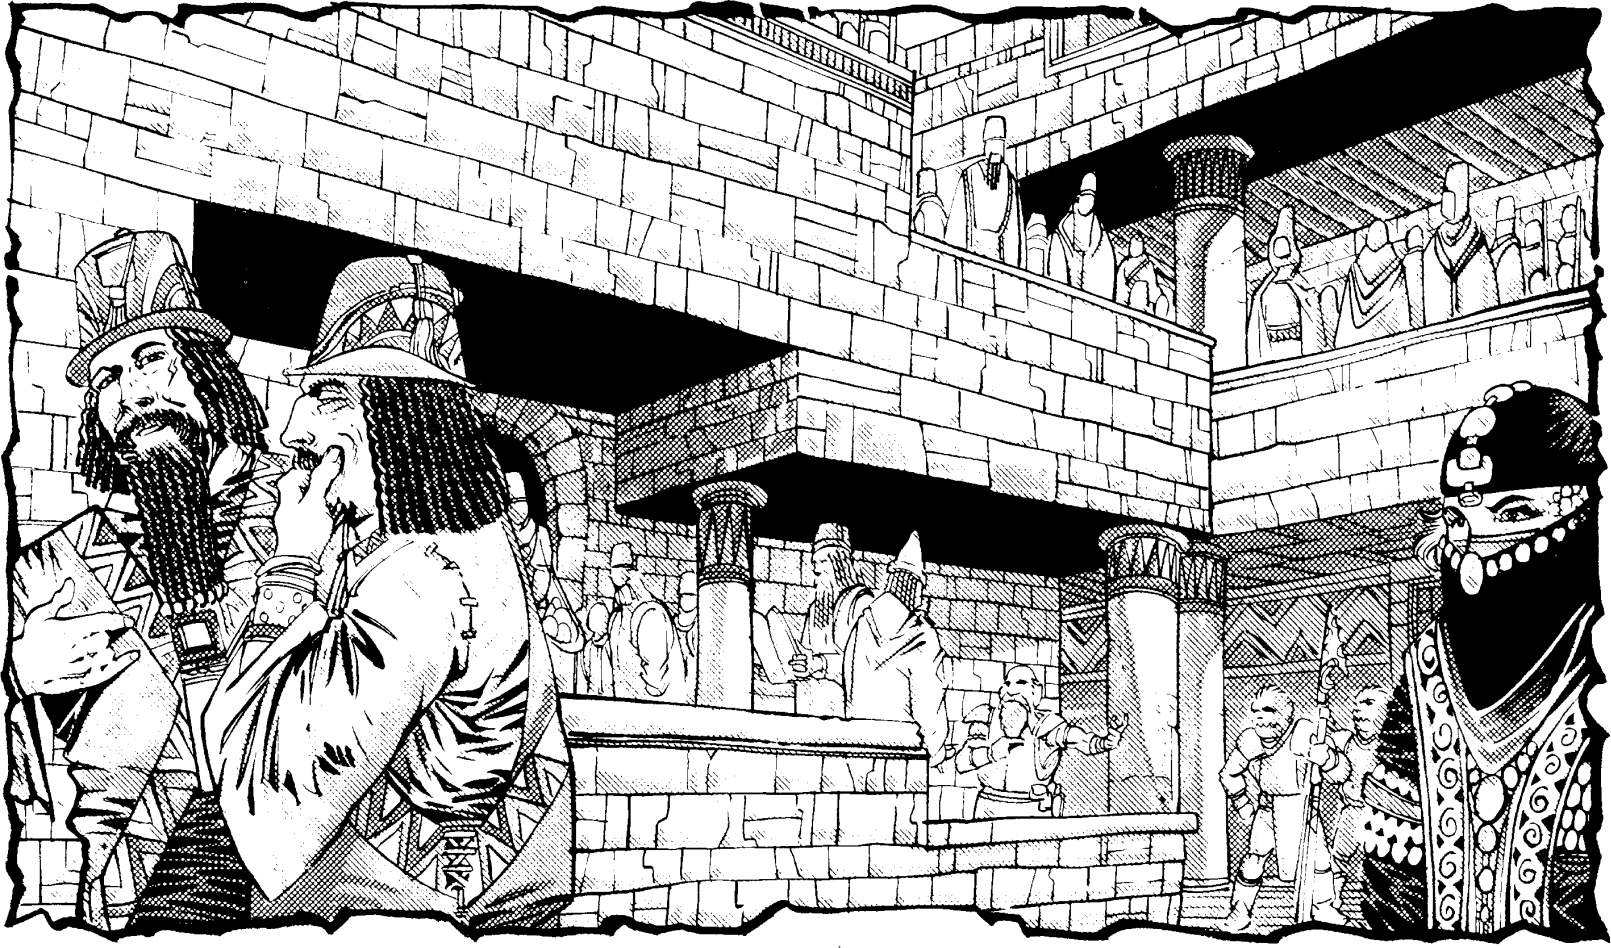
\includegraphics[width=\textwidth]{images/urik-2.png}
\par\textit{\small\textcopyright Wizards of the Coast, 2020.}
\end{figure*}

	The sorcerer-king Hamanu rules Urik, taking a personal interest in the affairs of his city. Except for Hamanu's direct involvement, Urik operates as a traditional sorcerer-king's domain. Templars enforce Hamanu's laws and handle the day-to-day bureaucracy, nobles manage the farms and water supplies, free citizens engage in business and try to remain free, and slaves provide the muscle to get everything else done.

	Hamanu is a third-stage dragon king (LE male Champion of Rajaat stage III dragon, defiler 5/psychic warrior 11/arch defiler 10/cerebremancer 5/Athasian dragon 4). Through a combination of the Way and magic, he appears before his subjects as either a tall, vigorous man with close-cropped silver hair, dark skin stretched tight over ruthless features, and heartless yellow eyes, or as a half-man and half-lion of powerful build and mythic proportions. He is never seen in his true dragon form, even by his most-trusted templars. His laws, called Hamanu's Code, are strict and innumerable, covering almost every conceivable aspect of life in Urik. Hamanu's Code relies on punishment in kind and emphasizes loyalty to the king and his templars. The Code stands unsurpassed in the Tyr Region for utility, comprehensiveness, and ruthlessness.

	At one time, Hamanu's ambitions exceeded his resources. Since the Great Earthquake and the events surrounding Rajaat's brief return, his agenda has subtly changed. The three surviving sorcerer-kings sensed that the time had come to rethink the old ways, to find new approaches to the challenges of life on Athas. Until he figures out what those new approaches are, Hamanu has decided to withdraw a bit. He has effectively closed Urik off from the rest of the Tablelands, trying to keep change from intruding on his domain for as long as possible.
}
{
	\textbf{The Brotherhood of the Mind}: The Brotherhood of the Mind is an organization of evil psionic-users that wish to overthrow the sorcerer-kings and seize power for themselves. Ruled by Liumakh, an undead psion, (NE male undead, telepath 10/thrallherd 7) the Brotherhood is headquartered in a monastery in the Smoking Crown mountains. Both Hamanu and Nibenay know of the brotherhood's existence. Nibenay seeks their destruction, while Hamanu ignores them for the most part, though he occasionally spies on the brotherhood to see if they have developed anything interesting during their psionic studies.

	\textbf{Hamanu's Halflings}: Hamanu has forged an agreement with a halfling chief from the Ringing Mountains. As long as Hamanu provides the chief with obsidian from the Urikite mines, he receives the services of 200 halfling warriors. These halflings are excellent night raiders and assassins that Hamanu has used to deadly effect in the past.

	\textbf{House Stel}: House Stel is best known for trading in the spoils of war, weapons, slaves, and various stolen cargo. Heavily influenced by the militant nature of Hamanu's regime in Urik, Stel is aggressive and confrontational with rivals. Stel caravans are heavily guarded to prevent against raids from other merchant houses, a tactic the house uses on its rivals regularly. The leaders of House Stel have a deep hatred of elves which has led to open warfare with a number of Elven tribes over the years. The House maintains lucrative trading contacts with halflings of the Ringing Mountains. Hargan Stel III (LN male human, fighter 5/rogue 2/ dune trader 5) leads the house and reflects the nature of his house, being both an expert trader and warrior.

	\textbf{The Veiled Alliance}: The Veiled Alliance has to be doubly careful in the wake of Hamanu's restrictions, and the preservers' supplies of spell components have become extremely limited. For most of the decade following the war with Tyr, Urik's Veiled Alliance was split into two factions. Its leader, the legendary Morlak, disappeared mysteriously, leaving two preservers to contend for the spot he vacated.

	When one of the contenders, Leoricius the Untamable, was killed in the Great Earthquake, the other contender worked feverishly to heal the split. This became increasingly important in the wake of Hamanu's newest restrictions. Today, Thania (LN female half-elf, preserver 5/veiled one 7) commands a whole Alliance, advocating patience and negotiation instead of the violent confrontations advocated by her one-time rival. Thania has been working to establish a partnership with Tyr's Alliance, but if Hamanu learns of it both groups will undoubtedly suffer.
}
{
	\textbf{Makla (Village, 1,000)}: The obsidian mines of Urik are located on the Mountain of the Black Crown, a peak in the Smoking Crown mountain chain. Urik's economy is completely dependent on obsidian and the tools fashioned from it. The Urikite client village of Makla serves as a base camp for the mining operations on Black Crown. The village is located on the shores of the Lake of Golden Dreams. Heavily fortified with over 500 guards, it is rarely attacked by raiders.

	\textbf{Fort Courage}: Fort Courage is a massive fortress on the trade road between Makla and Urik. This facility of House Stel is a supply point for caravans traveling between Urik and Makla and the halfling village of Ogo. Patrols are also sent from the fort to discourage raids on caravans along this route.
}
{
	\textbf{Destiny's Kingdom}: Sorcerer-King Hamanu rules Urik from his palace inside the massive fortress of Destiny's Kingdom. The walled fortress covers one square mile at the center of the city, containing troop barracks, drill fields, and an armory to support the army, as well as administrative offices for the king's templars.

	\textbf{The King's Academy}: The only legal psionic school in Urik is located within Destiny's Kingdom and is called the King's Academy. Students who attend the Academy are subject to a strict education that brings harsh punishment for failure. At the same time students are indoctrinated with the militarism that runs through the government of Urik.

	\textbf{Little Jungle}: A portion of the drill fields inside Destiny's Kingdom has been set aside for Hamanu's halfling allies to make their homes. Little Jungle is the name given to the fenced off area, where the halflings build huts in the jungle style.

	\textbf{Pit of Black Death}: Urik uses the site of an old obsidian mine for a gladiator arena, thus giving the arena its name, the Pit of Black Death. The Pit does not rise above the ground but is sunken into the ground. Stepped excavation provides viewing platforms for the crowd. All spectators must stand in the Pit, as there are no seats in the arena. The irregularly shaped combat area is made entirely of obsidian. The sun heats the black obsidian until it becomes almost unbearable for both combatants and spectators. As such most gladiator matches are held in the morning before the heat has become too great, or on rare occasions at night. Another danger of the obsidian is the thousands of sharp edges, shards, and spikes that protrude from the walls of the arena. These obsidian shards cover the walls and columns of obsidian that are scattered around the arena floor.

	\textbf{Potter's Court}: Pottery is an art form in Urik, and all other city-states recognize the superiority of Urikite pottery. The potters' workshops are collected in the Potter's Court area of the city. The concentration of so many immense kilns in the area, make Potter's Court unbearably warm, even at night when most of the potters conduct their work.

	\textbf{Potters' School}: The Potters' School is the largest group of psionic users who refuse to attend the King's Academy or register with the authorities. While the Potters' School teaches pottery casting and painting, skilled psions instruct students in the Way, outside of the influence of King Hamanu and his templars. The head instructor of the psions is Erriok (LN male human, shaper 7). He is rumored to have contact with the Veiled Alliance and work with them on occasion.

	\textbf{Three Sisters Observatory}: The Three Sisters Observatory is a two storey building with a flat roof and many observation balconies built on top of a hill called Sunrise Point. The Three Sisters Observatory served as the king's observatory until the construction of the Royal Observatory. Now the building is used to store old astronomical records and equipment, and has a run down, neglected appearance. The observatory gets its name from three identical granite hills nearby.
}
{
	\item Templars arrive at where the PCs are staying with orders to arrest them. Someone has accused the PCs of practicing magic. A fair trial is not possible and the sentence is death. The PCs must escape the templars, find out who their accuser is, and clear their name before they are captured by the templars.
	\item Unbeknownst to the PCs, their names have been added to a bounty list the templars of Urik maintain. Templars and bounty hunters begin to appear, trying to collect the bounty by capturing or killing the PCs. Whether or not the PCs are wanted by the templars, in this instance it is a case of mistaken identity. A wealthy merchant, wanted for smuggling, is supposed to be on the bounty list, however, he bribed a templar to remove his name and that of his family from the list. The PCs' names were chosen at random and added in place of the merchant's and his family to fill the vacancy.
	\item House Wavir has heard rumors that King Hamanu is planning on ordering his templars to seize all of their house's assets in Urik. Using the Wavir coup in Balic as an example, the house will be accused of planning a rebellion in Urik. Before he goes through with this threat, Hamanu is checking with the other major merchant-houses to gain their acceptance of his actions so they do not boycott his city. House Wavir gets wind of the plot and secretly plans to sneak out of the city with as much of their assets as possible. The PCs are hired to coordinate and have to safely get the Wavir agents and as much of their various assets, including wagons, merchandise, and draft animals, out of the city.
	\item The PCs are attending a feast at a noble's compound when the head of the family is murdered. Templars descend on the compound preventing anyone from leaving. Instead of investigating the crime, the templars simply state that unless the murderer is presented to them by morning everyone in the house will be executed. The PCs have until morning to find the real killer, or be executed along with everyone else.
	\item The Veiled Alliance has wondered for years about the high drik transformation process. The PCs are assigned to steal a drik egg that has undergone the process but that has not yet hatched.
	\item Saita, a templar of Urik, secretly sold some of the city's slaves to a tribe of yuan-ti in the Ringing Mountains to make some extra money. Unfortunately, the slaves were the personal property of Hamanu who is now enraged that his slaves are missing, and wants the head of the person responsible. Saita is desperate to get the slaves back before it is discovered that she is the one responsible. She secretly hires the PCs to get the slaves back from the yuan-ti any way they can.
}